%=========================================================================
% (c) 2011, 2012 Josef Lusticky

\section{Clock interface}
Previous section described how the call for getting the time acquires
the maximum precision the clock model allows.
Two read operations are needed in such a design - read {\it{scount}} and read {\it{TCNT2}}.
Since the {\it{scount}} variable depends on asynchronous interrupts produced by
the clock module, the followed query of the counter register causes a race condition.
The timer clock runs asynchronously from the CPU clock and
the result may be unpredictable if read while the timer is running.
Although the read could be wrapped with an interrupt disable,
the common solution on AVR platform in Contiki is to perform more read operations,
compare the results and perform read operations again if the results are not consistent.
Figure~\ref{fig:design-read} illustrates such a solution.

\begin{figure}
  \centering
  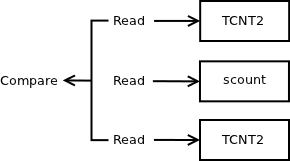
\includegraphics[width=6cm,keepaspectratio]{fig/read.png}
  \caption{Multiple read and result comparison}
  \label{fig:design-read}
\end{figure}

The call for adjusting the time computes the number of clock ticks
with longer or shorter tick interval.
When adjusting the time, the %TODO
as follows:

CLOCK\_COMPARE\_REGISTER = 30 => ca132.129Hz => 1s = ca1.032258s
FREQ = 32768/8 / 31
CLOCK\_COMPARE\_REGISTER = 32 => 124.12per => 1s = 0.96p
FREQ = 32768/8 / 33

Adjusting time - CLOCK\_COMPARE\_REGISTER = 31 => 128Hz => 1s = 1s
FREQ = 32768/8 / 32

The fastest adjust is 0.03 $\frac{s}{s}$.

% TO NTP INTERFACE
When writing to compare register, the value is transferred to a
temporary register, and latched after two positive edges of a source clock~\cite{avr-datasheet}.
The user should not write a new value before the contents
of the temporary register have been transferred to its destination.
To detect that a transfer to the destination register has taken place,
the Asynchronous Status Register - ASSR has been implemented.
Since writing to compare register occurs only once within interrupt CONTEXT, % context?
this detection is not mandatory.



This is enough for implementing a reasonable time interface and using it for NTP client later.

% ntp interface extending the clock library, similar to posix calls


Each TCNT2 increment is $\frac{1}{128 \times 32} \doteq 0,000244$s
0,244ms
This is also minimal possible clock adjustment.


Please note, that these adjustments will influence Contiki timers.
Applications requiring uninfluenced timers
are therefore advised to use rtimers, described in section~\ref{sec:contiki-timers},
because they use separate hardware clock unaffected by NTP client
(Timer/Counter~3 on AVR Raven platform).
